\thispagestyle{empty}
\chapter{Technical documentation} \label{appendix:technical-docs}
\pagenumbering{arabic}
\renewcommand*{\thepage}{C-\arabic{page}}

\section{Data collection plan}

The vibration measurements will occur monthly for pumps and biweekly for compressors from February 2024 until May 2024.
\begin{table}[ht]
\centering
\renewcommand{\arraystretch}{1.1}
\begin{tabular}{|l|l|p{0.6cm}|p{0.6cm}|p{0.6cm}|p{0.6cm}|p{0.6cm}|p{0.6cm}|}
\hline
\textbf{Machine}                                                                      & \textbf{Placement \textbackslash Month} & \multicolumn{2}{p{1.2cm}|}{\textbf{02/2024}} & \multicolumn{2}{p{1.2cm}|}{\textbf{03/2024}} & \multicolumn{2}{p{1.2cm}|}{\textbf{04/2024}} \\ \hline
\multirow{3}{*}{\textbf{\begin{tabular}[c]{@{}l@{}}Compressor\\ AC \#3\end{tabular}}} & SFTA001AT000TN                          &         &        &       &        &     &        \\ \cline{2-8} 
                                                                                      & SFTA002AT000TN                          &         &        &       &        &     &         \\ \cline{2-8} 
                                                                                      & Steel base (noise)                      &         &        &       &        &     &         \\ \hline
\multirow{3}{*}{\textbf{\begin{tabular}[c]{@{}l@{}}Compressor\\ AC \#5\end{tabular}}} & SFTA001AT000TN                          &         &        &       &        &     &         \\ \cline{2-8} 
                                                                                      & SFTA002AT000TN                          &         &        &       &        &     &         \\ \cline{2-8} 
                                                                                      & Steel base (noise)                      &         &        &       &        &     &         \\ \hline
\multirow{6}{*}{\textbf{\begin{tabular}[c]{@{}l@{}}Pump KSB\\ position \#1\end{tabular}}} & MTRA001AT090TN                          & \multicolumn{2}{p{1.2cm}|}{}                 & \multicolumn{2}{p{1.2cm}|}{}                 & \multicolumn{2}{p{1.2cm}|}{}                 \\ \cline{2-8} 
                                                                                      & MTRA002AT000TN                          & \multicolumn{2}{p{1.2cm}|}{}                 & \multicolumn{2}{p{1.2cm}|}{}                 & \multicolumn{2}{p{1.2cm}|}{}                 \\ \cline{2-8} 
                                                                                      & PMPA003AT000TN                          & \multicolumn{2}{p{1.2cm}|}{}                 & \multicolumn{2}{p{1.2cm}|}{}                 & \multicolumn{2}{p{1.2cm}|}{}                 \\ \cline{2-8} 
                                                                                      & PMPA004AT000TN                          & \multicolumn{2}{p{1.2cm}|}{}                 & \multicolumn{2}{p{1.2cm}|}{}                 & \multicolumn{2}{p{1.2cm}|}{}                 \\ \cline{2-8} 
                                                                                      & Motor base (noise)                      & \multicolumn{2}{p{1.2cm}|}{}                 & \multicolumn{2}{p{1.2cm}|}{}                 & \multicolumn{2}{p{1.2cm}|}{}                 \\ \cline{2-8} 
                                                                                      & Pump base (noise)                       & \multicolumn{2}{p{1.2cm}|}{}                 & \multicolumn{2}{p{1.2cm}|}{}                 & \multicolumn{2}{p{1.2cm}|}{}                 \\ \hline
\multirow{6}{*}{\textbf{\begin{tabular}[c]{@{}l@{}}Pump KSB\\ position \#7\end{tabular}}} & MTRA001AT090TN                          & \multicolumn{2}{p{1.2cm}|}{}                 & \multicolumn{2}{p{1.2cm}|}{}                 & \multicolumn{2}{p{1.2cm}|}{}                 \\ \cline{2-8} 
                                                                                      & MTRA002AT000TN                          & \multicolumn{2}{p{1.2cm}|}{}                 & \multicolumn{2}{p{1.2cm}|}{}                 & \multicolumn{2}{p{1.2cm}|}{}                 \\ \cline{2-8} 
                                                                                      & PMPA003AT000TN                          & \multicolumn{2}{p{1.2cm}|}{}                 & \multicolumn{2}{p{1.2cm}|}{}                 & \multicolumn{2}{p{1.2cm}|}{}                 \\ \cline{2-8} 
                                                                                      & PMPA004AT000TN                          & \multicolumn{2}{p{1.2cm}|}{}                 & \multicolumn{2}{p{1.2cm}|}{}                 & \multicolumn{2}{p{1.2cm}|}{}                 \\ \cline{2-8} 
                                                                                      & Motor base (noise)                      & \multicolumn{2}{p{1.2cm}|}{}                 & \multicolumn{2}{p{1.2cm}|}{}                 & \multicolumn{2}{p{1.2cm}|}{}                 \\ \cline{2-8} 
                                                                                      & Pump base (noise)                       & \multicolumn{2}{p{1.2cm}|}{}                 & \multicolumn{2}{p{1.2cm}|}{}                 & \multicolumn{2}{p{1.2cm}|}{}                 \\ \hline
\multirow{6}{*}{\textbf{Pump Sigma}}                                                  & MTRA001AT000TN                          & \multicolumn{2}{p{1.2cm}|}{}                 & \multicolumn{2}{p{1.2cm}|}{}                 & \multicolumn{2}{p{1.2cm}|}{}                 \\ \cline{2-8} 
                                                                                      & MTRA002AT000TN                          & \multicolumn{2}{p{1.2cm}|}{}                 & \multicolumn{2}{p{1.2cm}|}{}                 & \multicolumn{2}{p{1.2cm}|}{}                 \\ \cline{2-8} 
                                                                                      & PMPA003AT000TN                          & \multicolumn{2}{p{1.2cm}|}{}                 & \multicolumn{2}{p{1.2cm}|}{}                 & \multicolumn{2}{p{1.2cm}|}{}                 \\ \cline{2-8} 
                                                                                      & PMPA004AT000TN                          & \multicolumn{2}{p{1.2cm}|}{}                 & \multicolumn{2}{p{1.2cm}|}{}                 & \multicolumn{2}{p{1.2cm}|}{}                 \\ \cline{2-8} 
                                                                                      & Motor base (noise)                      & \multicolumn{2}{p{1.2cm}|}{}                 & \multicolumn{2}{p{1.2cm}|}{}                 & \multicolumn{2}{p{1.2cm}|}{}                 \\ \cline{2-8} 
                                                                                      & Pump base (noise)                       & \multicolumn{2}{p{1.2cm}|}{}                 & \multicolumn{2}{p{1.2cm}|}{}                 & \multicolumn{2}{p{1.2cm}|}{}                 \\ \hline
\end{tabular}
\end{table}
Each measurement will involve 3 trials for each position. The sensor is mounted to the machine with adhesive on double-sided carpet tape (placement notation follows MIMOSA convention from ISO~13373-1). After every trial, the sensor will be detached and attached again. 

The plan was consulted and approved by the machinery owners: VNET~a.s. and Bratislavská vodárenská spoločnosť,~a.s. Triaxial recording has a duration 60~s (at $f_s$ = 26.7 kHz) and a 16-bit resolution. The total space requirements for 108 recordings are 990 MiB.

\section{Firmware activities}
Activity diagrams describe three basic actions of firmware for logging accelerometer samples:

\begin{itemize}
\itemsep0pt
\item begin new recording, 
\item log block of samples into CSV file,
\item finish recording.
\end{itemize}

\begin{figure}[h]
    \centering
	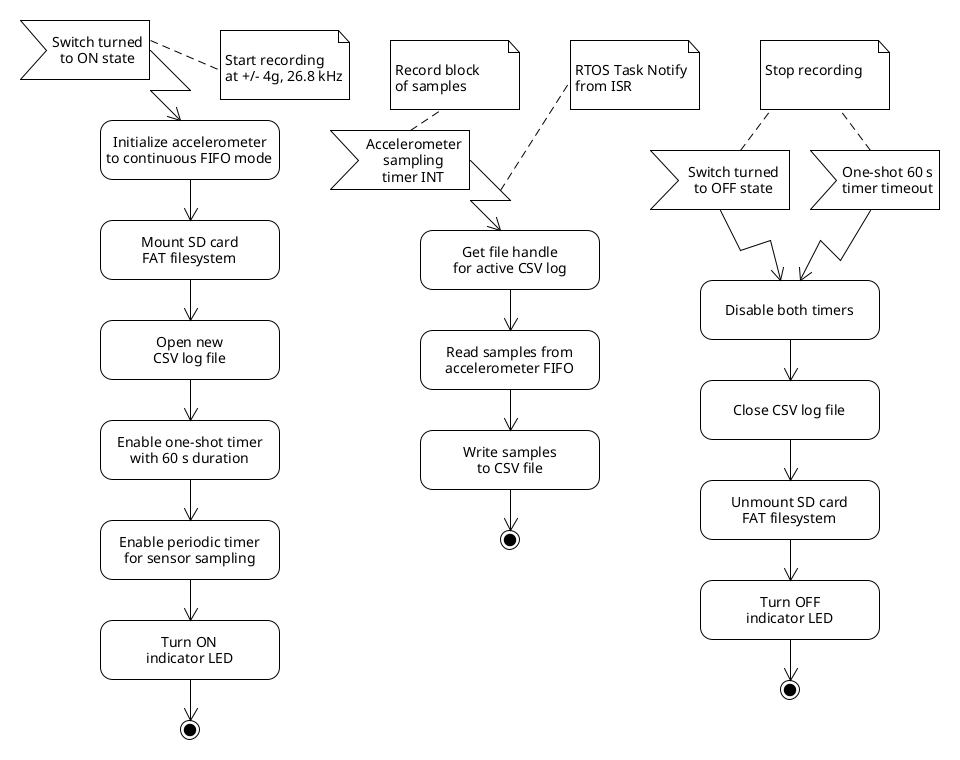
\includegraphics[width=\textwidth]{assets/design/firmware-design.png}
\end{figure} 
